\documentclass[sigconf]{acmart}

\usepackage{booktabs} % For formal tables
\usepackage{amsmath}
\usepackage{tipa}
\usepackage{subcaption}
\usepackage{graphicx}
\usepackage{hyperref}
\usepackage{parskip}
\usepackage{minted}
\usepackage{xcolor}
\usepackage{listings}
\usepackage{color}
 
\definecolor{codegreen}{rgb}{0,0.6,0}
\definecolor{codegray}{rgb}{0.5,0.5,0.5}
\definecolor{codepurple}{rgb}{0.58,0,0.82}
\definecolor{backcolour}{rgb}{0.95,0.95,0.92}
 
\lstdefinestyle{mystyle}{
    backgroundcolor=\color{backcolour},   
    commentstyle=\color{codegreen},
    keywordstyle=\color{magenta},
    numberstyle=\tiny\color{codegray},
    stringstyle=\color{codepurple},
    basicstyle=\footnotesize,
    breakatwhitespace=false,         
    breaklines=true,                 
    captionpos=b,                    
    keepspaces=true,                 
    numbers=left,                    
    numbersep=5pt,                  
    showspaces=false,                
    showstringspaces=false,
    showtabs=false,                  
    tabsize=2
}
 
\lstset{style=mystyle}

% Copyright
\setcopyright{none}
%\setcopyright{acmcopyright}
%\setcopyright{acmlicensed}
%\setcopyright{rightsretained}
%\setcopyright{usgov}
%\setcopyright{usgovmixed}
%\setcopyright{cagov}
%\setcopyright{cagovmixed}


% DOI
\acmDOI{ }

% ISBN
\acmISBN{ }

%Conference
\acmConference[DTU]{DTU conference}{August 2017}{Kgs Lyngby, Denmark} 
\acmYear{1997}
\copyrightyear{2017}


\acmArticle{1}
\acmPrice{3.50}

% These commands are optional
%\acmBooktitle{Transactions of the ACM Woodstock conference}
%\editor{Roar Nind Steffensen}


\begin{document}
\title{Report 2 - Operating Systems}
%\titlenote{Produces the permission block, and copyright information}
\subtitle{Roar Nind Steffensen (s144107)}
%\subtitlenote{The full version of the author's guide is available as
%  \texttt{acmart.pdf} document}


%\author{Ben Trovato}
%\authornote{Dr.~Trovato insisted his name be first.}
%\orcid{1234-5678-9012}
%\affiliation{%
%  \institution{Institute for Clarity in Documentation}
%  \streetaddress{P.O. Box 1212}
%  \city{Dublin} 
%  \state{Ohio} 
%  \postcode{43017-6221}
%}
%\email{trovato@corporation.com}

% The default list of authors is too long for headers.
%\renewcommand{\shortauthors}{B. Trovato et al.}


%\begin{abstract}
%This paper provides a sample of a \LaTeX\ document which conforms, somewhat loosely, to the formatting guidelines for ACM SIG Proceedings.\footnote{This is an abstract footnote}
%\end{abstract}

%
% The code below should be generated by the tool at
% http://dl.acm.org/ccs.cfm
% Please copy and paste the code instead of the example below. 
%
%\begin{CCSXML}
%<ccs2012>
% <concept>
%  <concept_id>10010520.10010553.10010562</concept_id>
%  <concept_desc>Computer systems organization~Embedded systems</concept_desc>
%  <concept_significance>500</concept_significance>
% </concept>
% <concept>
%  <concept_id>10010520.10010575.10010755</concept_id>
%  <concept_desc>Computer systems organization~Redundancy</concept_desc>
%  <concept_significance>300</concept_significance>
% </concept>
% <concept>
%  <concept_id>10010520.10010553.10010554</concept_id>
%  <concept_desc>Computer systems organization~Robotics</concept_desc>
%  <concept_significance>100</concept_significance>
% </concept>
% <concept>
%  <concept_id>10003033.10003083.10003095</concept_id>
%  <concept_desc>Networks~Network reliability</concept_desc>
%  <concept_significance>100</concept_significance>
% </concept>
%</ccs2012>  
%\end{CCSXML}

%\ccsdesc[500]{Computer systems organization~Embedded systems}
%\ccsdesc[300]{Computer systems organization~Redundancy}
%\ccsdesc{Computer systems organization~Robotics}
%\ccsdesc[100]{Networks~Network reliability}


%\keywords{Processes, Threads, System Calls, C}

\maketitle

The implementation for weeks 5, 6 and 7 will be uploaded in the zip file: \texttt{s144107skeletons567.zip}.

\section{Week 5}
%\begin{itemize}
    
    %\item Draw a figure of the organization of the system.
    %\item Relate the organization of the system to the different types of operation systems discussed in the text book by Tanenbaum and Bos.
    %\item What kind of operating system is it? Why?
    %\item How is the system booted? Outline each step.
    
%\end{itemize}

\subsection{The system skeleton}

The system as given in the skeleton is composed of some start up files such as \texttt{entry.s}, defining the environment and certain low level protocols. This involves, disabling interrupts, clearing any statically allocated variables, setting up the kernel stack, and further down the line, call \texttt{kernel\_init} found in \texttt{kernel.c}. The \texttt{startup\_32.s} file contains the protocol for starting a program, setting up the needed environment, and calling the respective main function. The kernel implementation is seen in the \texttt{kernel} and \texttt{kernel\_customization} files, together with the \texttt{video.c} file defining how information is displayed on the monitor. In the labs, we are mainly concerned with the development of the file \texttt{video.c} together with the \texttt{kernel\_customization} header and \texttt{c} file. 

\begin{figure}[H]
    \centering
    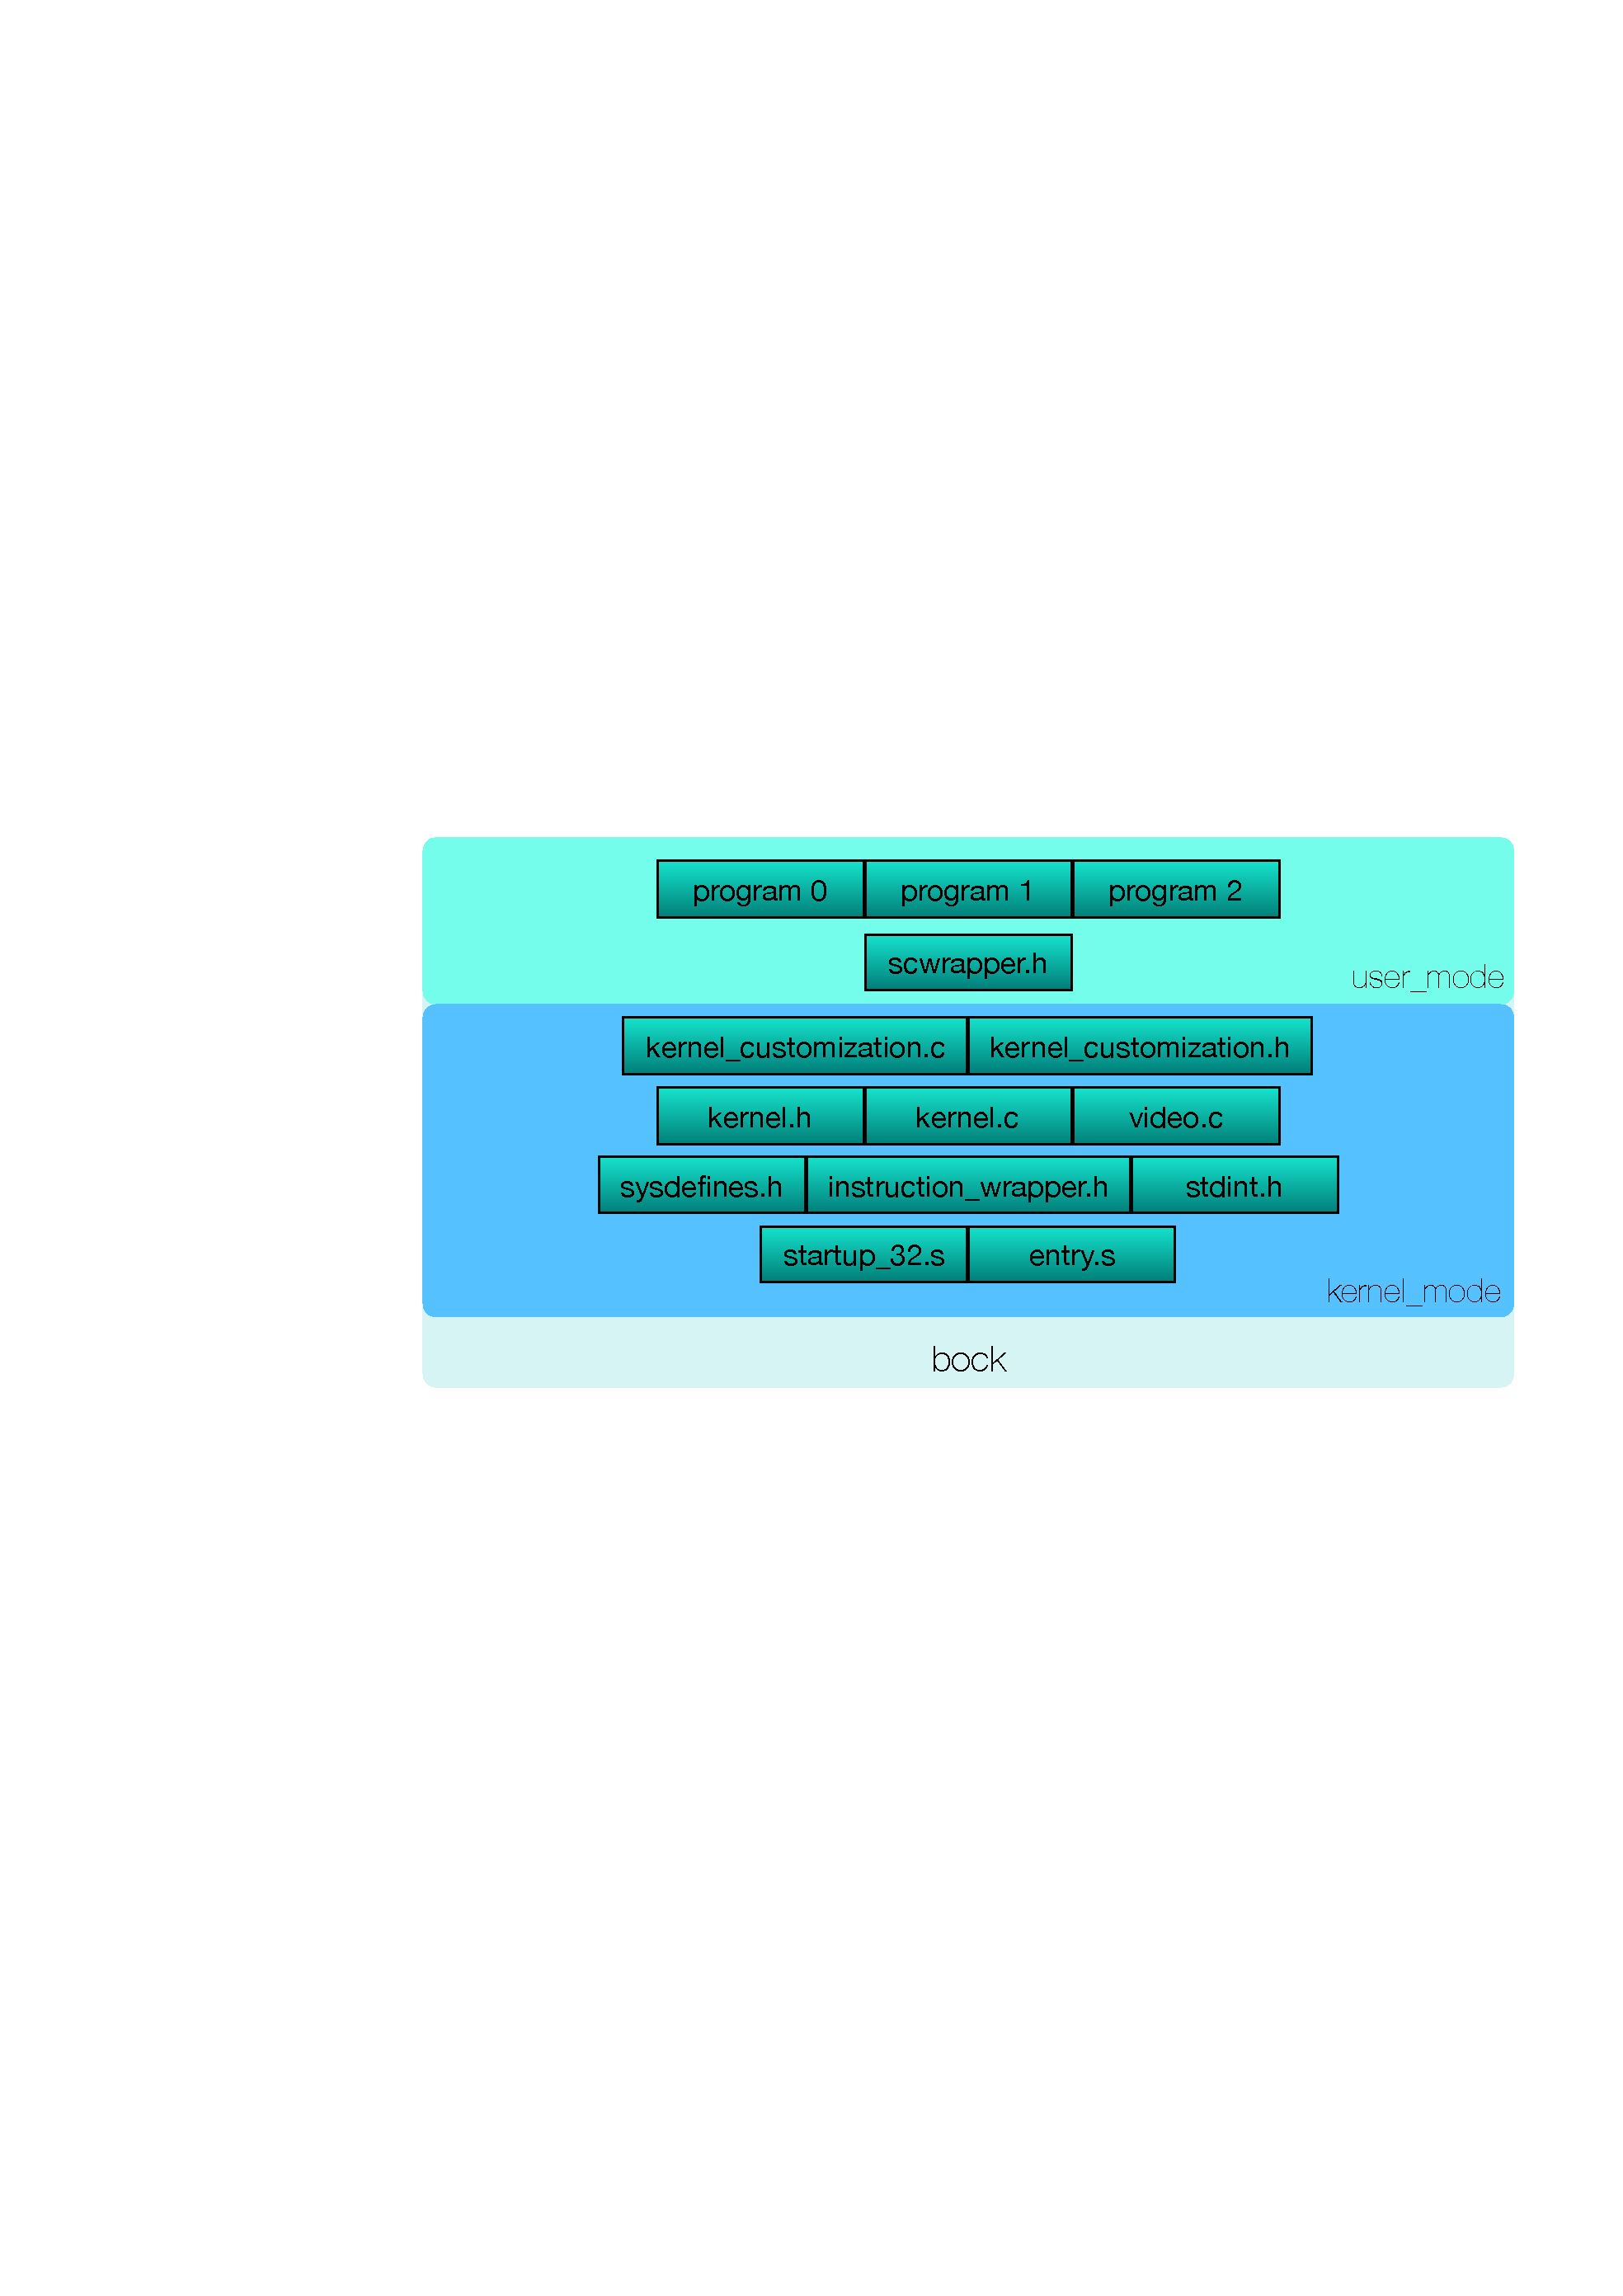
\includegraphics[width=\linewidth]{fig/system_organization.pdf}
    \caption{Organization of the system implementation.}
    \label{fig:sys_org}
\end{figure}

The programs run in \texttt{user\_mode}, and in order to call system calls executed in \texttt{kernel\_mode}, the \texttt{scwrapper.h} acts as a trap, switching to \texttt{kernel\_mode} using the assembly call \texttt{sysenter} and passing the appropriate parameters on the current threads registers. The \texttt{sysenter} entry point protocol is executed in \texttt{entry.s} which calls the \texttt{handle\_system\_call} function implemented in the file \texttt{kernel\_customization.c}. Once the system call has executed, the system returns to \texttt{user\_mode}, and the program continues. 


Other files like \texttt{instruction\_wrappers.h}, \texttt{sysint.h} and \texttt{sysdefines.h} contain macros, type definitions and assembly instruction wrappers accessible to the kernel. The layering of these implementations are outlined in figure \ref{fig:sys_org}.

Since the different system calls and kernel operations are implemented inside the kernel, this is not a micro-kernel operating system. All resource management is handled through system calls, and not directly, meaning this is not an exo-kernel operating system, which means, that we in fact have a monolithic operating system. For a monolithic operating system, all kernel operations are accessible within \texttt{kernel\_mode}, which is also what we experience in our system. 

In figure \ref{fig:sys_org} we have \texttt{boch} at the very bottom, since this is the program simulating our system in which we launch the operating system. Boch itself is close enough to the actual hardware that the operating system may have access directly to hardware, meaning that the bottom layer could be replaced with hardware.

\section{Week 6}

\subsection{System calls}

%\begin{itemize}
    
    %\item Where are system calls implemented? Hint: Have a look in kernel customization.c.

    
%\end{itemize}

\textbf{System call implementations} \\
The heart of the system calls is implemented in the kernel, more specifically the \texttt{kernel\_customization.c} file. Here a function called \texttt{handle\_system\_call} is called which in turn executes the procedure as specified by the value from the \texttt{eax} register. This way, the system call handle acts as a finite automata, only acting based on the system call, as seen in figure \ref{fig:syscall_imp}. Other parameters may be read from the different registers depending on what system call is specified. The return statement is also placed on the \texttt{eax} register, generally specifying if the procedure was executed successfully or not.

\begin{figure}[H]
    \centering
    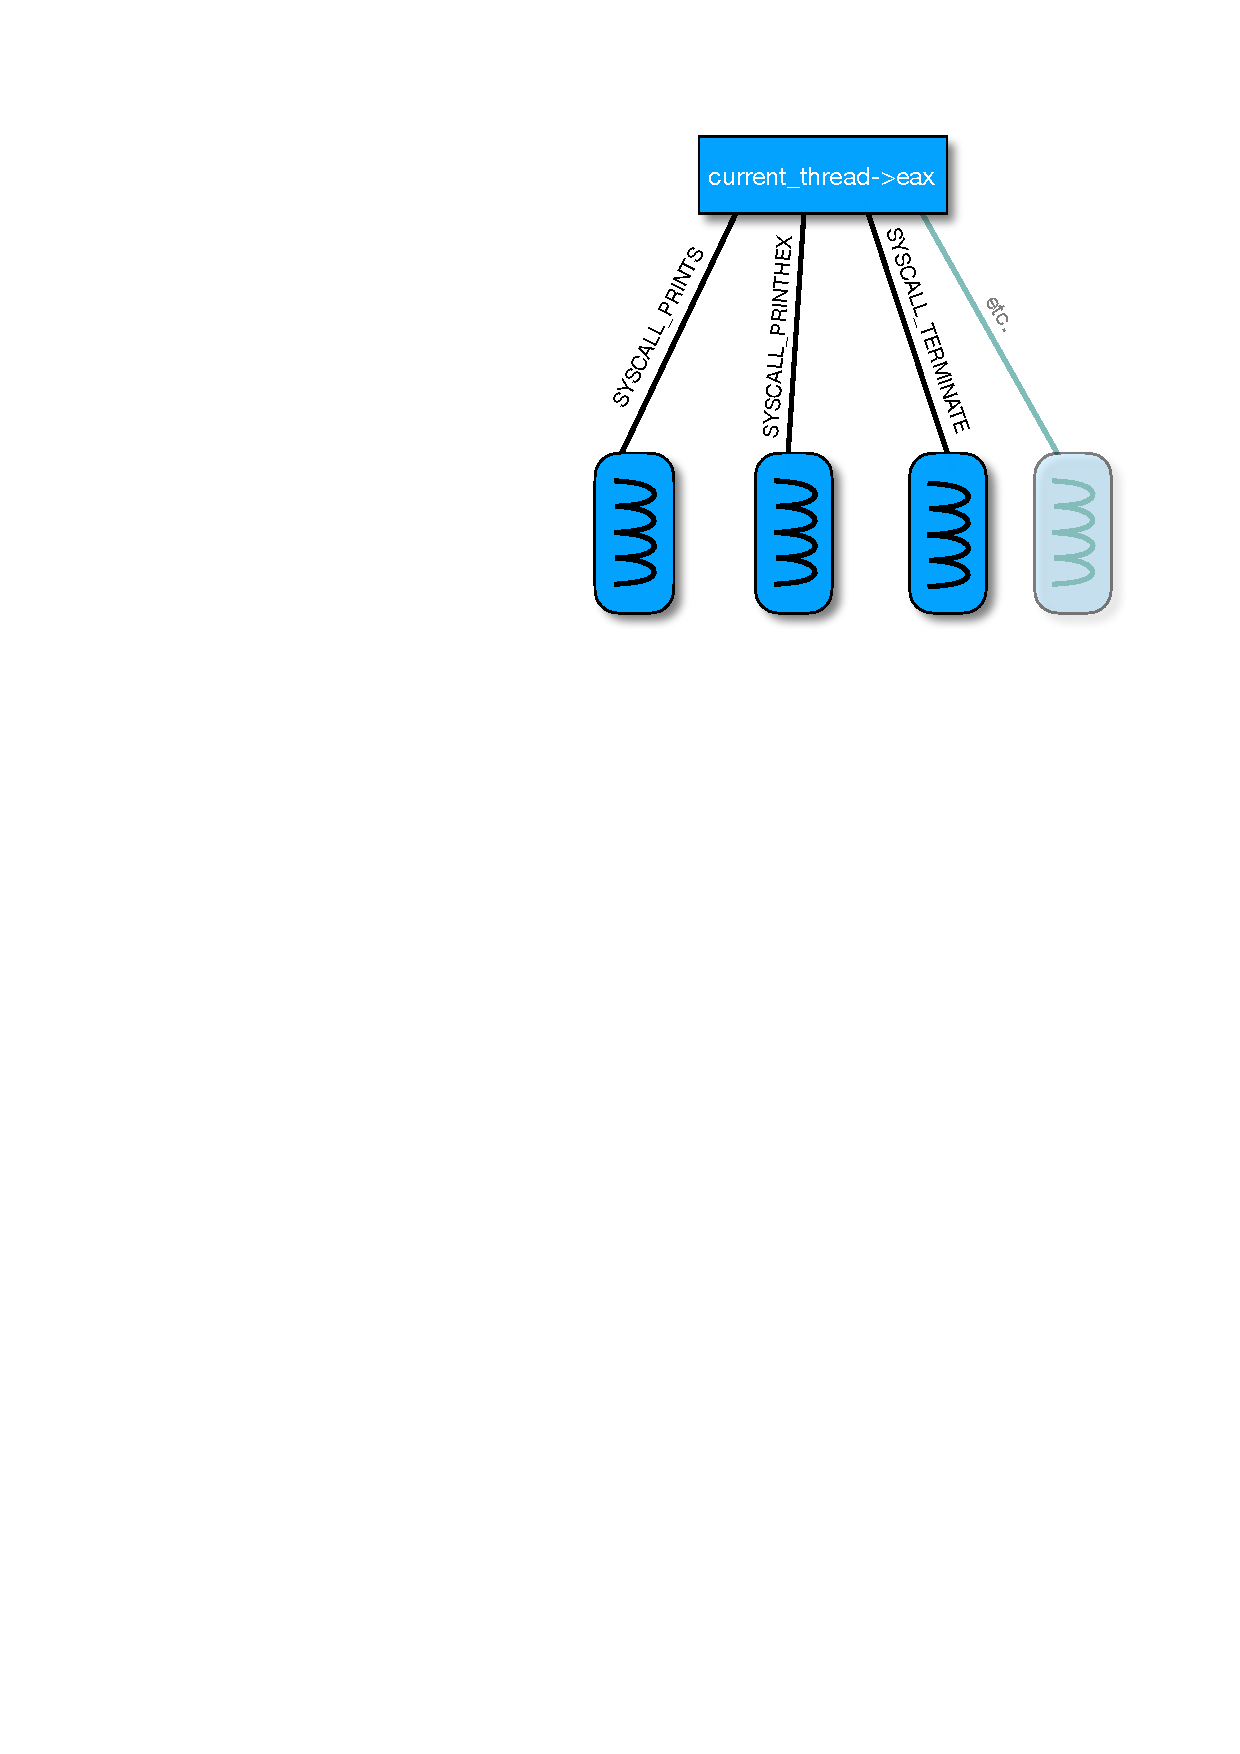
\includegraphics[width=0.7\linewidth]{fig/systemcall_implementation.pdf}
    \caption{System call handler, depicted as a finite automata.}
    \label{fig:syscall_imp}
\end{figure}

An example of a system call implementation is given as follows:

\begin{lstlisting}[language=c, caption=System call example]
void handle_system_call(void)
{
switch (current_thread->eax)
 {
  case SYSCALL_VERSION:
  {
   current_thread->eax = 0x00010000;
   break;
  }
  default:
  {
   /* Unrecognized system call. Not good. */
   current_thread->eax = ERROR_ILLEGAL_SYSCALL;
  }
 }
 go_to_user_space();
}
\end{lstlisting}

This clearly shows how the case statements of the switch corresponds to the states in the finite automata in figure \ref{fig:syscall_imp}, and the edge depends on the value of the \texttt{eax} register. Hitting the default case of the switch corresponds to a state in the automata receiving a symbol which does not match an edge. Instead of a stuck or crash, we return an error.

\subsection{Processes}
%\begin{itemize}
    
    %\item What is the purpose of the current thread variable?
    
    %\item The processes array?
    
    %\item The threads array?
    
    %\item How are threads and processes represented?
    
    %\item How many simultaneous processes can there be? Why?
    
    %\item How many simultaneous threads can there be? Why?
    
    %\item In the current skeleton, what data, in a wide sense, can at all be associated with processes?

%\end{itemize}

\textbf{The current thread variable} \\
Since the operating system is designed to have multiple processes able to contain multiple threads, the \texttt{current\_thread} variable is used as a pointer to the thread currently executing. 

\textbf{The processes array} \\
The \texttt{processes} array allocates memory for the possible processes available to have running at the same time in the operating system. The array also functions as a table to look up different processes e.g. for the scheduler. 

Each process is kept as a struct containing the number of threads held and system flags used by the scheduler. 

The length of the array dictates how many processes can run simultaneously, which is 16 as specified by the variable \texttt{MAX\_PROCESSES} in the \texttt{kernel} header file.

\textbf{The threads array} \\
The \texttt{threads} array acts much like the \texttt{processes} array as it also allocates memory for the possible threads available to have running at the same time while functioning as a look up table.

Each thread is kept as a struct containing the variables corresponding to the 7 registers available, a process pointer to identify the responsible process and system flags, again used by the scheduler.

The length of the array dictates how many threads can run simultaneously, which is 256 as specified by the variable \texttt{MAX\_THREADS} also in the \texttt{kernel} header file.

The sizes of the two arrays are a power of two, which may be efficient for future scheduling algorithms, which may utilize heaps or trees. Also there are more threads than processes, each process at least needs one thread, but can use multiple if needed. All 16 processes can each have 16 threads, but a single process can also use all 256 threads.

\subsection{Non-preemptive scheduling}
The scheduler in this system is implemented using a \texttt{simple round} robin algorithm which circles the thread array and finds a thread which is used by a process. This ensures, that each time \texttt{yield} is called, all other threads are evaluated before the initial thread continues, making it intrinsically fair. 

A more efficient approach could be to store the requesting threads in a FIFO queue, meaning that inactive threads are not evaluated.

Since the threads are a power of two, the threads array could be used as a max-heap sorted by priority. This the next thread would always be on the top of the heap while changing priority of a thread would at most cost $\log_2(256)=8$ operations. To maintain the max-heap structure.

\subsection{Process termination}

%\begin{itemize}
    %\item The skeleton code actually calls terminate after a user "main" returns. Where is that done? Hint: Have a look in the "C library", the startup 32.s file.

    %\item How would you change the user programs so at least one program terminates?
%\end{itemize}

\textbf{Terminate procedure} \\
In the \texttt{startup32.s} file we see the setup procedure for programs run in the operating system. The stack pointer is set to the value of the \texttt{esp} register of the thread. Values \texttt{argv} and \texttt{argc} containing an array of strings (program name as first element) and the amount of elements in the array respectively are pushed on stack for the main function. In this case just one element in the string array. Then the main function of the program is called. When the main function returns we finally set the value of the \texttt{eax} register to 6, corresponding to the \texttt{SYSCALL\_TERMINATE} value as registered in the \texttt{sysdefines} header file. The system call then handles termination of the thread, and frees any resources from the thread. If the thread is the only thread of it's process, the process is also terminated. Since threads and process are stored statically in arrays, terminating a thread and/or a process is done by setting the system flags \texttt{used} to 0, telling the scheduler that they are no longer active. 

For other programs to continue when a thread has terminated, \texttt{yield} is called, informing the scheduler that a new thread can continue executing. If no other threads/processes are active, the scheduler cannot direct the flow to a new thread, and the system does not proceed. 
\begin{lstlisting}[language=c, caption=System call terminate]
case SYSCALL_TERMINATE:
{
 current_thread->used = 0;
 struct process* current_process=current_thread->process;
 if(current_process->number_of_threads != 0)
 {
   current_process->number_of_threads--;
   kprints("Thread terminated\n");
 }
 if(current_process->used == 1 && current_process->number_of_threads == 0)
 {
   kprints("Process terminated");
   current_process->used = 0;
 }
 current_thread->eax = SYSCALL_YIELD;
 handle_system_call();
 break;
} 
\end{lstlisting}
An alternative could be to call \texttt{halt\_the\_machine} to stop the machine.

\textbf{Terminating a user program} \\
In order to terminate a user program either the \texttt{terminate} function can be called, or the while loop in the program can be removed in order to reach the end of the function. Both actions call the terminate system call setting the \texttt{SYSCALL\_TERMINATE} on the \texttt{eax} register which in turn gets handled in the switch found in \texttt{kernel\_customization.c}.

\subsection{Reflection questions}

\textbf{Steps in executing a system call}\\
The specific steps of a system call depends on the implementation of the operating systems, in this case we will focus on the procedure in the skeleton from the labs. This has already briefly been outlined in section \textbf{The system skeleton}.

From user-mode, a function is called from the \texttt{scwrapper.c}, which initializes the environment for the system call to proceed. If arguments are passed to the function, e.g. a string for printing, or an integer creating a process to execute a specific program from the execution table, this is set into appropriate \texttt{edi} or \texttt{esp} register of the current thread. The \texttt{id} for system call itself is placed on the \texttt{eax} register, using specified values in the \texttt{sysdefines} header file. The "sysenter" call is performed, invoking the \texttt{system\_call\_handler} function. This acts as a trap, going from user-mode to kernel-mode, where the implementation of the system call is handled, as mentioned in the \textbf{System call implementations} section. Once the system call has finished, the system returns to user-mode and the return value for the initial function call is extracted from the \texttt{eax} register of the current thread.

\textbf{Daemon processes}\\
A daemon (process) is a program which runs in the background. This could be used e.g. for notifications, auto-saving the state, collecting emails, maintaining an internet connection and such. Daemon processes are highly efficient at dividing the workload, and removing delay from the main processes. By providing services in the background, the user does not need to wait for e.g. a document to save while the interaction with the system is frozen. This strategy is efficient not only for performance, but also for user experience.

\textbf{Scheduler}\\
The main job of a scheduler is to control which processes/threads are allowed to execute operations. Depending on the implementation, either the scheduler differentiates between processes or threads when choosing which job to run. For our labs the scheduler works with threads, since the our kernel does not support parallel execution by multiple cores on the CPU. If parallel executions were supported, a process would be preferred to run with its threads in parallel. If the process contains more threads than cores, the scheduler would control the flow between the process' threads. Possibly by a two layer scheduler, a higher layer for process scheduling and a lower layer for thread scheduling within processes.

The scheduling algorithm implemented in our labs is mentioned in the \textbf{Non-preemptive scheduling} section.

\textbf{Thread states}\\
The different states of a thread are; \textit{running}, \textit{blocked}, \textit{ready}. These states are implemented as follows:\\
\textit{running}: A thread is \textit{running} if it is status flag \texttt{used} is 1 and the thread is chosen by the scheduler. \\
\textit{blocked}: A thread is \textit{blocked} if it is terminated, as seen by the status flag \texttt{used} being 0. It will not be chosen by the scheduler.\\
\textit{ready}: A thread is \textit{ready} if the status flag \texttt{used} 1 but it has not yet been chosen by the scheduler.

The transitions between these states correspond to the transitions in figure 2-2 in the Tanenbaum book \cite{tanembaum}. A running thread can be be ready or blocked, either by yielding or termination respectively. A ready thread can be running by being chosen by the scheduler. A blocked thread can be ready by being "created" by a process (by another thread). 

\textbf{Preemptive system}\\
Currently the implementation forces the individual threads to yield if they should be allowed to run concurrently. This is because we have a non-preemptive system. For a system to be preemptive, a process is given a time frame (a quantum) to run in, after which it is interrupted (forced to yield) and another process is scheduled. For this to work, the scheduler must be activated when the time is due for a new process to run, possibly by a clock interrupt. This way, the work load may be more evenly and fairly distributed across processes, which is highly desirable when multiple processes are running at the same time, since no one of them gains monopoly on the CPU time.

%\begin{itemize}
    %\item What are the steps in executing a system call?
    
    %\item How are parameters to system calls passed to the operating system?
    
    %\item How is the kernel mode entered? How do you return to user space?
    
    %\item How does a daemon (process) differ from processes studied in this assignment?
    
    %\item What is a scheduler? What does it do and how does it work?
    
    %\item Assume a thread can be in three different states: running, blocked, ready. Between the states, there are various transitions. Relate the states and transitions to the code and actions in the system.
    
    %\item How does preemption influence the design of an operation system? How does it influence the scheduler?

%\end{itemize}
\section{Week 7}

\subsection{Threads}

The concept of multiple threads per process is now introduced to the operating system. In order to see how this is handled, we first have to outline how processes are created.

Creating a process is done by the following steps:
\begin{itemize}
    \item Find a process not in use.
    \item If no process was found, return \texttt{ERROR}.
    \item Find a thread not in use.
    \item If no thread was found, return \texttt{ERROR}.
    \item If both process and thread was found, update them and return \texttt{ALL\_OK}.
\end{itemize}

For the final step, the process' and thread's \texttt{used} flags are set to 1, the process' count of inner threads is set to 1, the thread's inner process pointer is set to the found process and the thread's instruction pointer is set to the value in the \texttt{execution\_table} corresponding to the program assigned. 

This way a new process is created and assigned the program given. The process has a single thread, and only if both the process and thread were created does the system call return \texttt{ALL\_OK}.

Creating a thread is a similar case, accept we don't need to find a process, since it will be assigned to the current thread's process. The steps are then condensed into:

\begin{itemize}
    \item Find a thread not in use.
    \item If no thread was found, return \texttt{ERROR}.
    \item If thread was found, update it and return \texttt{ALL\_OK}.
\end{itemize}

Where updating the thread involves setting the \texttt{used} flag to 1, the process is set to the current thread's process, the inner thread count of the process is incremented and the thread's instruction and stack pointers are set to the given values from registers \texttt{edi} and \texttt{esi} of the current thread.

Since the scheduler already schedules jobs by threads, no change is needed to control this new feature.

\bibliographystyle{ACM-Reference-Format}
\bibliography{sample-bibliography} 

\end{document}
